\documentclass[a4paper, 15pt]{article}
\usepackage[left=0.85in, right=0.85in, top=0.5in, bottom=0.95in]{geometry}
\usepackage[T1]{fontenc}
\usepackage[utf8]{inputenc}
\usepackage[italian]{babel}

% Formattazione del testo
\usepackage{setspace}         % Setting dello spazio\begin{spacing}{0.95}
\setstretch{1.2}
\setlength{\parindent}{0pt}
\raggedbottom
\usepackage[none]{hyphenat}    % no sillabazione 
\usepackage{multicol}          % testo su più colonne
\usepackage{changepage}	       % \begin{adjustwidth}{}{}

% Matematica
\usepackage{amsmath, amssymb, amsthm, mathtools}
\usepackage{cancel}            % semplificazioni \cancel{expression}
\newtheorem*{thm}{Teorema}
\newtheorem*{en}{Enunciato}
\newtheorem*{definizione}{Definizione}
\newtheorem*{cor}{Corollario}
\DeclareMathOperator{\rk}{rk}
\DeclareMathOperator{\im}{Im}

% Simboli e Disegni
\usepackage{color}             % \textcolor{'ColorCode'}{'testo'}
\usepackage{graphicx, wrapfig, float}
\usepackage{tikz, circuitikz}
\usetikzlibrary{patterns, arrows, decorations.markings, arrows.meta, decorations.text}
\tikzset{immagine/.style={above right, inner sep=0pt, outer sep=0pt},
	testo/.style={fill=white, align=center, fill opacity=0.6, text opacity=1, below, font=\sffamily\bfseries\footnotesize}}
\usepackage{pgfplots}
\pgfplotsset{compat=1.15}
\usepackage{mathrsfs}

% Altri pacchetti
\usepackage{enumitem}
\usepackage{mdwlist} 	       % suspend enumerate \suspend{} \resume{}
\usepackage{siunitx}
\usepackage{hyperref}
\hypersetup{
	colorlinks=true,
	linkcolor=blue,    
	urlcolor=blue,
}
\urlstyle{same}

% Altre definizioni personali
\usepackage{pifont}
\newcommand{\cmark}{\ding{51}}
\newcommand{\xmark}{\ding{55}}
\DeclareUnicodeCharacter{20AC}{\EUR}
\newcommand{\compresslist}{\setlength{\itemsep}{1pt}\setlength{\parskip}{0pt}\setlength{\parsep}{0pt}}
\newcommand{\ra}[1]{\renewcommand{\arraystretch}{#1}} % stretcho le tabelle e gli array \ra{x}
\setlength{\jot}{10pt}


% Titolo e data
\title{10. Misure di portata e velocità per ifluidi}
\date{}

\begin{document}
	\maketitle
	\setcounterpageref{secnumdepth}{0}
	\setcounter{tocdepth}{5}  % Includo nel TOC anche i subsubpar	
	\tableofcontents 
	\newpage
	
	
	
%\end{adjustwidth}
%\newpage
\section{Misure di portata}
\begin{adjustwidth}{2in}{}	
	Un fluido scorre in un condotto a causa di una differenza di pressione
	esistente fra due diverse sezioni.
	
	La portata volumetrica rappresenta il volume di fluido che
	attraverso la sezione considerata nell’unità di tempo
	\[\dot{Q} = \dfrac{dV}{dt} = [\si{\metre\cubic\per\second}]\]
	Esprimendo il volume come una sezione per una lunghezza si ottiene
	che la portata può essere vista come il prodotto tra una sezione e una
	velocità.
	
	Se al posto del volume si fa riferimento alla massa, si parla di
	portata massica
	\[\dot{m} = \dfrac{dm}{dt} = \rho\dfrac{dV}{dt} = [\si{\kilogram\per\second}]\]
	
	I trasduttori per la misura di portata possono essere suddivisi in due categorie:
	\begin{itemize}
		\item\underline{A restringimento di sezione / A strozzamento} 
		
		Se si basano sull'introduzione di un restringimento nella sezione di passaggio del fluido causando un decremento della pressione statica (perdita di carico): la misura della portata avviene sempre grazie al $\Delta P$ imposto, non è mai una misura diretta.
		
		\item \underline{NON a strozzamento}
		
		Se si basano su principi differenti come il bilancio di quantità di moto, o ultrasuoni \dots		
	\end{itemize}
	A prescindere dal principio fisico i trasduttori per la misura di portata
	vengono chiamati \textbf{flussometri}. 
\end{adjustwidth}
%\newpage
\subsection{Flussometri a strozzamento}
\begin{adjustwidth}{2in}{}	
	\begin{itemize}
		\item \textbf{Diaframmi}: di semplice realizzazione e basso ingombro, inducono importanti perdite di carico >20\% causate dal distacco della vena fluida e dall'instaurarsi di un moto fortemente turbolento.
		
		\item \textbf{Boccaglio}: per flussi di vapore ad elevata velocità, presenta un tratto convergente al fine di guidare i filetti fluidi, riduce le perdite di carico intorno al 15\%.
		
		\item \textbf{Boccaglio - Venturi}: presenza di un tratto convergente-divergente, con dimensioni inferiori ad un venturimetro.
		
		\item \textbf{Venturimetri}: il tratto convergente è un cilindro a sezione costante mentre il tratto divergente presenta un piccolo angolo di conicità. 
		
		Le perdite di carico possono ridursi fino ad arrivare al 2\%, tuttavia può raggiungere dimensioni ragguardevoli, dai \SI{16}{\metre} di lunghezza con \SI{4.5}{\metre} di diametro.		
	\end{itemize} 
\end{adjustwidth}
%\newpage
\subsubsection{Venturimetro}
\begin{adjustwidth}{2in}{}	
	\begin{figure}[H]
		\centering
		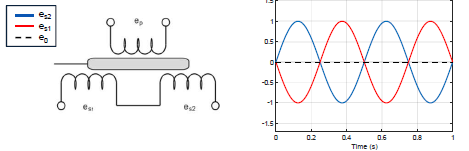
\includegraphics[width=0.3\linewidth]{immagini/screenshot001}
		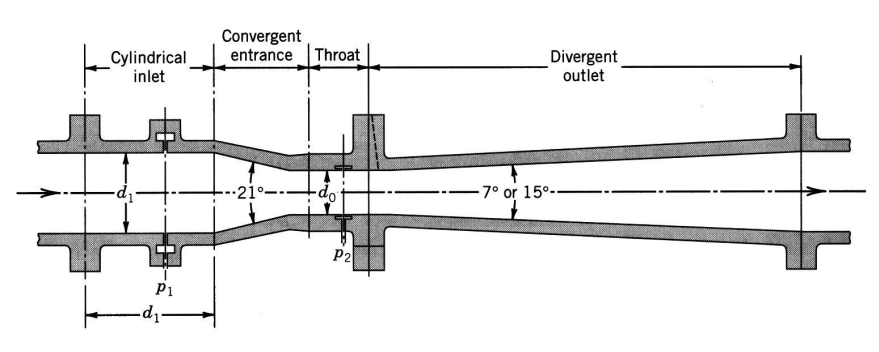
\includegraphics[width=0.5\linewidth]{immagini/screenshot002.1}
		\label{fig:screenshot001}
	\end{figure}
	Il graduale aumento di sezione dopo il tratto convergente permette una diminuzione delle perdite di carico ma comporta un maggiore ingombro. \newline 
	
	L'equazione che governa il venturimetro è l'equazione di continuità, questa infatti garantisce che la portata - per fenomeni stazionari - è costante in ogni sezione
	\[\dot{Q} = S_1v_1 = S_2v_2\]
	Per fluidi incomprimibili se $S_2<S_1$ si ha dalle equazioni di Hugoniot che $v_2>v_1$. 
	
	Applicando il teorema di Bernoulli tra le sezioni, dopo aver verificato le sue ipotesi di applicabilità, si perviene a 
	\[P_1 + {1\over2}\rho v_1^2 = P_2 + {1\over2}\rho v_2^2\]
	La differenza di pressione diviene così esprimibile come 
	\[P_1-P_2 = {1\over2}\rho(v_2^2-v_1^2)\]
	Si può risalire così alla velocità conoscendo la differenza di pressione, misurabile. 
	
	Si definisce a questo punto il coefficiente di strozzamento come 
	\[Z = \dfrac{S_2}{S_1}<1\]
	In modo che la conservazione della portata si possa riscrivere come 
	\[v_1 = \dfrac{S_2}{S_1}v_2 = Zv_2\]
	Questa sostituita nell'equazione di Bernoulli ricavata porta a 
	\[\Delta P = {1\over2}\rho v_2^2(1-Z^2)\]
	Da cui la velocità 
	\[v_2^2 = \dfrac{2\Delta P}{\rho(1-Z^2)}\]
	E la portata volumetrica diviene così pari a 
	\[\dot{Q} = S_2v_2 = S_2\sqrt{\dfrac{2\Delta P}{\rho(1-Z^2)}}\]
	La differenza di pressione è misurabile attraverso un manometro differenziale collegato alle due prese di pressione. \newline 
	
	Per un fenomeno reale le perdite di carico non possono essere trascurate, per cui si dovrà tener conto di un coefficiente di efflusso
	\[C = \dfrac{\dot{Q}_{id}}{\dot{Q}_{re}}<1\]
	Questo, non costante, dipenderà dal numero di Reynolds $Re$ secondo tabelle fornite dal costruttore. \newline 
	
	L'equazione finale per il calcolo della portata diviene così 
	\[\dot{Q} = CS_2\sqrt{\dfrac{2\Delta P}{\rho(1-Z^2)}}\]
	Notare come sia uno strumento fortemente non lineare dalla sensibilità non costante: è più alta nella zona finale del campo di misura, il venturimetro è adatto per elevati valori di portata.
	\begin{itemize}[label = \textcolor{red}{\xmark}]
		\item Costo elevato
		\item Ingombro elevato dovuto alla lunghezza del tratto divergente, questo infatti non può superare i 15\unit{\degree} al fine di evitare distacchi di vena fluida
		\item Perdite di carico (seppur minime).
		
		Alla fine del tratto divergente non tutto il carico di pressione viene
		recuperato, si verifica quindi un errore di inserzione
		\begin{figure}[H]
			\centering
			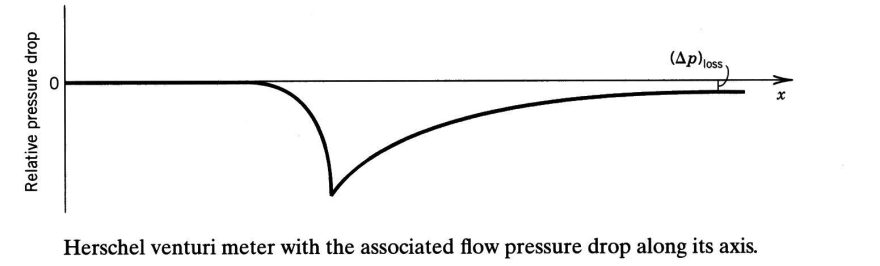
\includegraphics[width=0.5\linewidth]{immagini/screenshot002.2}
			\label{fig:screenshot002}
		\end{figure}		
	\end{itemize}
\end{adjustwidth}
%\newpage
\subsubsection{Flussometro a galleggiante - Rotametro}
\begin{adjustwidth}{2in}{}	
	\begin{figure}[H]
		\centering
		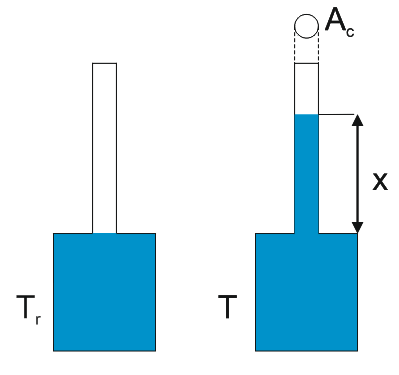
\includegraphics[width=0.5\linewidth]{immagini/screenshot003}
		\label{fig:screenshot003}
	\end{figure}
	È uno strumento di facile costruzione che permette il
	raggiungimento di accuratezza elevata (1\%).
	
	È costituito da un tubo di vetro o materiale plastico trasparente dalla forma lievemente troncoconica, \textbf{quasi} a strozzamento, su cui è incisa esternamente una scala di "graduazione". 
	
	Al sui interno è collocato un galleggiante di materiale e di forma opportuni allo scopo.
	
	Viene inserito in posizione verticale sul tubo di erogazione del fluido.
	
	Ha un campo di misura molto vasto: dal decimo di litro
	a migliaia di litri al secondo e non ha bisogno di un manometro differenziale per la
	misura della pressione.  
	
	\paragraph{Funzionamento} \mbox{} \\
	\begin{enumerate}
		\item Quando non vi è passaggio di fluido $(Q=0)$ il galleggiante è
		adagiato sul fondo del tubo.
		
		\item Al passaggio del fluido il galleggiante viene
		sollevato dal flusso e, a seconda della portata evolvente, si posizionerà ad
		una certa altezza in corrispondenza della quale l’operatore legge
		direttamente il valore della portata sulla scala graduata.
	\end{enumerate}
	
	Il principio fisico su cui si basa il rotametro è legato alla semplice relazione di equilibrio tra la forza peso del galleggiante nel fluido e la spinta stessa del fluido.\newline 
	
	Il \underline{peso del galleggiante} nel fluido vale
	\[P_g = (\rho_g-\rho_{fluido}) g V_g\]
	
	Mentre la \underline{spinta del flusso} sarà data, proprio dalla definizione, come sezione massima del galleggiante per la pressione a cui è sottoposta
	\[S = A(P_1-P_2)\]
	La differenza di pressione tra testa e piede del galleggiante, che contribuisce al suo sollevamento, sussiste in virtù della forma del galleggiante stesso.\newline 
	
	Dall'equilibrio delle forze si ha così
	\[(\rho_g-\rho_{fluido}) g V_g = A(P_1-P_2)\]
	Da cui
	\[\Delta P = \dfrac{\Delta \rho gV_g}{A}\]
	Da questa equazione si nota immediatamente come la differenza di pressione sia
	costante perché 
	\begin{enumerate}
		\item È funzione di parametri costanti 
		\item Non dipende dalla quota raggiunta dal galleggiante
	\end{enumerate} 	
	Applicando infatti la conservazione dell'energia (NB: il galleggiante è totalmente immerso nel fluido) ci si riconduce a 
	\[\Delta P = {1\over2}\rho_{fluido}v^2\]
	La velocità $v$ è relativa alla sezione anulare di passaggio del fluido che
	si viene a creare tra il galleggiante e il tubo troncoconico ed è anch'essa costante per qualunque quota raggiunta. \newline 
	
	Sostituendo questo risultato nell'equazione precedente si ha
	\[{1\over2}\rho_{fluido}v^2 = \dfrac{\Delta \rho gV_g}{A}\]
	Da cui
	\[v = \sqrt{\dfrac{2\Delta \rho gV_g}{A\rho_{fluido}}} = \sqrt{\dfrac{2gV_g}{A}\cdot\dfrac{\rho_g-\rho_{fluido}}{\rho_{fluido}}}\]
	E la portata sarà così pari a 
	\[\dot{Q} = CSv = CS\sqrt{\dfrac{2gV_g}{A}\cdot\left(\dfrac{\rho_g}{\rho_{fluido}}-1\right)} \]
	Tuttavia, dalla sua relazione, si nota che la velocità è costante: come si può allora misurare una portata? 
	
	Attraverso il cambio di sezione: al variare di $\dot{Q}$ deve variare la sezione anulare $S$, ecco perché il flussometro ha una forma troncoconica.
\end{adjustwidth}
%\newpage
\subsubsection{Flussometro a turbina}
\begin{adjustwidth}{2in}{}	
	\begin{figure}[H]
		\centering
		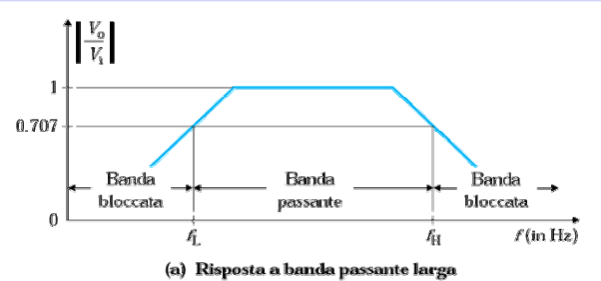
\includegraphics[width=0.3\linewidth]{immagini/screenshot004}
		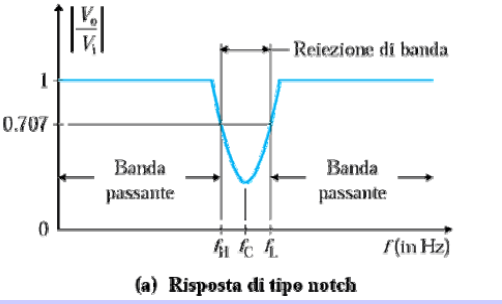
\includegraphics[width=0.5\linewidth]{immagini/screenshot005}		
		\label{fig:screenshot004}
	\end{figure}
	Il flussometro a turbina misura quanto velocemente ruota la turbina, il limite metrologico di questo strumento risiede nell'inerzia della turbina, per cui se la portata è troppo bassa questa non la mette in rotazione: è uno strumento del II ordine. \newline 
	
	Si presenta come un cilindro contente una girante il cui asse è sostenuto da due cuscinetti.
	
	Il cilindro esterno presenta due estremità filettate per l’inserimento nella
	linea idraulica in esame.
	
	A monte e a valle della girante possono essere presenti dei
	raddrizzatori di flusso che servono per guidare il flusso in direzione
	assiale.
\newpage
	\paragraph{Funzionamento} 
	\begin{figure}[H]
		\centering
		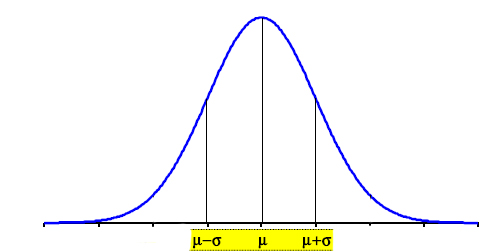
\includegraphics[width=0.5\linewidth]{immagini/screenshot006}
		\label{fig:screenshot006}
	\end{figure}
	La fisica che c'è dietro riguarda i triangoli di velocità. 
	\begin{itemize}
		\item $c$ velocità assiale, responsabile della portata 
		\item $w$ velocità relativa
		\item $u$ velocità tangenziale
	\end{itemize}
	Per cui, dalla trigonometria è facile realizzare che 
	\[\dfrac{u}{c} = \tan\alpha \Rightarrow c = \dfrac{u}{\tan\alpha} = \dfrac{\omega r}{\tan\alpha}\]
	In cui $\alpha$ è noto grazie al raddrizzatore, questo infatti ha il preciso compito di rendere il fluido più assiale possibile in modo da diminuire l'entità della velocità relativa.\newline 
	
	Dall'equazione di continuità ci si riconduce a 
	\[\dfrac{dV}{dt} = c\pi\dfrac{d^2}{4} = \dfrac{\pi\omega d^3}{8\tan\alpha} = \dfrac{\pi^2fd^3}{4\tan\alpha}\]
	Dove $f$ è la frequenza.
	
	Ciò significa che la portata transitante diviene nota conoscendo la frequenza di rotazione della girante, significa allora che a valle del sistema di misura dovrà esserci un oscilloscopio, o un frequenzimetro, o un encoder che ad ogni giro invii un segnale digitale. \newline 
	
	Il grosso limite di questo strumento è l'\textbf{inerzia meccanica}, a causa infatti delle irreversibilità meccaniche dei cuscinetti e della massa della girante, è necessaria una portata consistente affinché questa si metta in rotazione. 
	
	Il modello matematico descritto vale quando sussiste la relazione
	\[\dfrac{\rho_{fluido}\omega d^3}{\mu}>1000\]
\end{adjustwidth}
\newpage
\section{Misure di velocità}
\subsection{Tubo di Pitot}
\begin{adjustwidth}{2in}{}	
	Il tubo di Pitot è un trasduttore per la misura della velocità di un flusso
	portante.
	\begin{figure}[H]
		\centering
		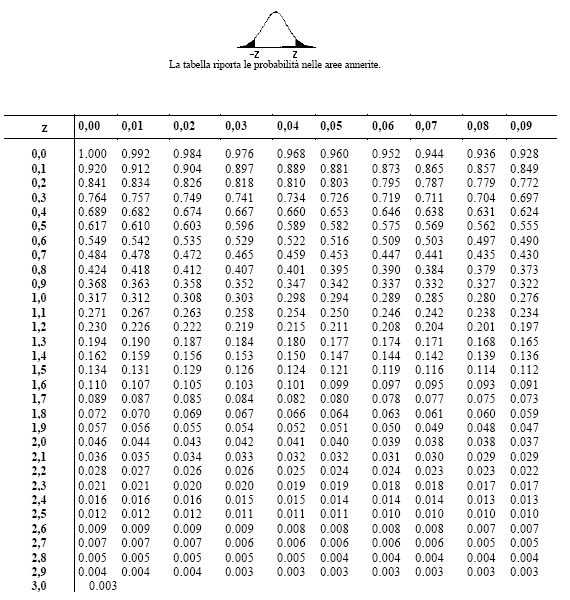
\includegraphics[width=0.5\linewidth]{immagini/screenshot007}
		\label{fig:screenshot007}
	\end{figure}
	
	Si presenta come una sonda cilindrica con un foro assiale che costituisce la presa totale (ristagno) e una serie di fori sul profilo
	laterale per la presa statica. 
	
	\paragraph{Funzionamento}
	\begin{figure}[H]
		\centering
		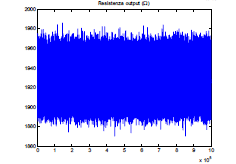
\includegraphics[width=0.5\linewidth]{immagini/screenshot008}
		\label{fig:screenshot008}
	\end{figure}
	Si consideri un fluido in moto laminare nel punto A. \newline 
	
	Nella sezione $S_1$ il fluido scorre indisturbato a velocità $v$. 
	
	Nella generica sezione $S_2$ il fluido entra invece in contatto con il trasduttore e questo comporta una deviazione di traiettoria con velocità finale del flusso pari a 
	\[w = v + v_f\]
	Con $v_f$ componente di frenamento. \newline 
	
	Si applichi il teorema di Bernoulli alle sezioni generiche
	\[S_1\rightarrow E_{tot} = P_{st} + {1\over2}\rho v^2 \qquad S_2\rightarrow E_{tot} = P + {1\over2}\rho w^2\]
	Dalla conservazione dell'energia si ricava che 
	\[P_{st} + {1\over2}\rho v^2 = P + {1\over2}\rho w^2\]
	Allora 
	\[\Delta P = {1\over2}\rho(v^2-w^2)\]
	Che si può riscrivere, introducendo il coefficiente di pressione $K_p$
	\[\Delta P = {1\over2}\rho(1-K_p) \qquad K_p = \dfrac{w^2}{v^2}\]
	Tale coefficiente di pressione è un parametro fondamentale per la scelta del corretto posizionamento della presa statica e di quella dinamica
	\begin{itemize}
		\item \(K_p = 1\)
		
		Il massimo del coefficiente di pressione si ha quando tutta la velocità del fluido viene frenata. 
		
		Ciò accade solamente all’inizio
		del sondino in corrispondenza dell’asse. 
		
		In questo punto infatti la pressione del fluido è massima: è qui che si deve posizionare la presa di pressione totale (ristagno).
		
		\item \(K_p = 0\)
		
		Il minimo del coefficiente di pressione si ha quando il flusso è indisturbato, senza componente di frenamento.
		
		Ciò accade ad una distanza di $5\div6$ diametri dall’inizio del sondino.
		
		In questo punto tutta la pressione del fluido è solamente di tipo statico: è qui che si deve posizionare la presa di pressione statica.
	\end{itemize}
	Identificate le posizioni corrette delle prese dinamica e statica, il sondino può immediatamente essere utilizzato in accoppiamento ad
	un manometro differenziale, per effettuare misure di velocità del fluido.
	\[\Delta P = {1\over2}\rho v^2\]
	
	\begin{itemize}[label = \textcolor{green}{\cmark}]
		\item Economico
		\item Di facile realizzazione 
		\item Assenza di perdite di carico grazie alla dimensioni estremamente contenute
	\end{itemize}
	
	\begin{itemize}[label = \textcolor{red}{\xmark}]
	\item Difficoltà di allineamento con la direzione del fluido
	\item Basse accuratezze (si usano infatti TdP ridondanti negli aeromobili)
	\end{itemize}
\end{adjustwidth}
%\newpage
\subsection{Anemometro a filo caldo}
\begin{adjustwidth}{2in}{}	
	\begin{figure}[H]
		\centering
		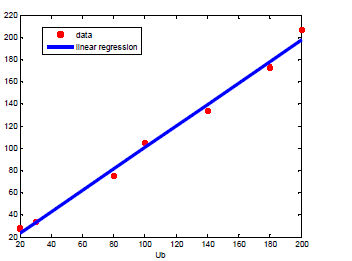
\includegraphics[width=0.1\linewidth]{immagini/screenshot009}
		\label{fig:screenshot009}
	\end{figure}
	
	L’anemometria è una tecnica ad alta risoluzione molto utilizzata per la misura della velocità dei fluidi.
	
	L’anemometro a filo caldo è lo strumento più diffuso. \newline
	
	Il principio fisico si basa sullo scambio termico tra fluido e filo che avviene per convezione, esiste infatti una relazione  tra il coefficiente di scambio termico per convezione $(h)$ e la velocità del fluido in cui il filo è
	immerso. 
\newpage
	Nel campo industriale per valutare lo scambio termico tra un filo sottile
	e la corrente fluida che lo investe in direzione trasversale si utilizza la
	seguente relazione
	\[Nu = A + B \cdot Re^n\]
	Un cui 
	\begin{itemize}
		\item $Nu$ è il numero di Nusselt
		\[Nu = \dfrac{hD}{k}\]
		\item $Re$ è il numero di Reynolds
		\[Re = \dfrac{\rho\nu D}{\mu}\]
		\item $A,B$ costanti dipendenti dal fluido in esame
		\item $D$ dimensione caratteristica
		\item $k$ conducibilità termica del fluido
		\item $\rho$ densità del fluido
		\item $\nu$ viscosità dinamica del fluido
		\item $v$ velocità assoluta del fluido
		\item $n$ nel campo di applicazione industriale può essere considerato pari a
		0.5
	\end{itemize}
	Ne consegue che la relazione finale tra coefficiente di scambio
	termico per convezione e velocità del fluido è
	\[h = C_1 + C_2\sqrt{v}\]
	
	Si supponga a questo punto di far scorrere una corrente elettrica nel filo dello strumento (realizzato in metallo puro). 
	
	Temperatura e resistenza elettrica del filo dipenderanno da $I$ corrente, $T_f$ temperatura del fluido e $h$ coefficiente di convezione. 
	
	La relazione di Newton per lo scambio termico per convezione si può scrivere quindi come 
	\[RI^2 = hA(T_s - T_f)\]
	Dove $A$ è la superficie di scambio termico e $T_s$ è la temperatura dello strumento, del filo.\newline 
	
	Sostituendo il coefficiente $h$ si arriva a 
	\[RI^2 = (C_1 + C_2\sqrt{v})A(T_s - T_f)\]
	Per poter calcolare la velocità, nell'ipotesi che $T_f$ non varii, si può scegliere di mantenere costante o l'intensità di corrente o la temperatura del filo. \newline
	
	\textbf{RICORDA}: l'anemometro a filo caldo è uno strumento attivo!  
\end{adjustwidth}
\newpage
\subsubsection{Anemometro a temperatura costante}
\begin{adjustwidth}{2in}{}		
	Lo schema circuitale di un anemometro a filo caldo a temperatura costante è quello mostrato in figura
	\begin{figure}[H]
		\centering
		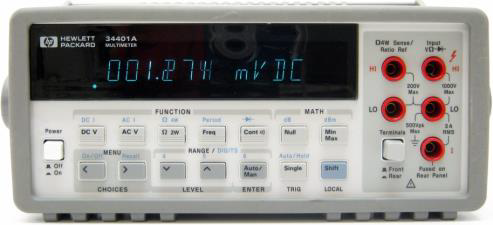
\includegraphics[width=0.3\linewidth]{immagini/screenshot010}
		\label{fig:screenshot010}
	\end{figure}
	In condizioni di equilibrio vale 
	\[I^2 = C_3+C_3\sqrt{v}\]
	Al variare della velocità del fluido varia la corrente necessaria affinché la temperatura del filo, e quindi la resistenza, rimanga
	costante.
	
	La corrente che scorre sul filo allora varia facendo variare $R_r$
	
	La nuova corrente crea così uno squilibrio del ponte che viene azzerato andando a variare $R_b$ attraverso una lettura col galvanometro G attraverso il metodo di zero. \newline
	
	A questo punto, a ponte azzerato, si procede alla lettura del valore $I$ che scorre sul filo.
	
	Ora si può procedere ad una taratura dello strumento per diversi valori di velocità $v$. 
	\begin{figure}[H]
		\centering
		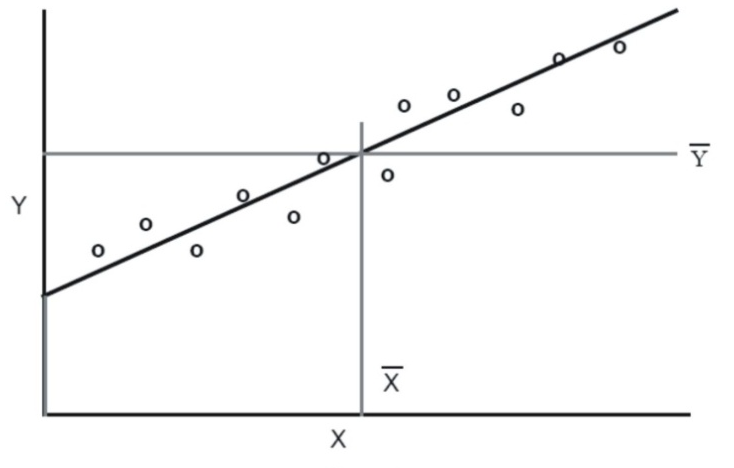
\includegraphics[width=0.2\linewidth]{immagini/screenshot011}
		\caption{L'anemometro a filo caldo è uno strumento lineare}
		\label{fig:screenshot011}
	\end{figure}
	
	\begin{itemize}[label = \textcolor{green}{\cmark}] \compresslist
		\item Ingombri bassissime con conseguente ridotto errore di inserzione (strumento del I ordine)
		\item Elevata banda passante: Strumento molto rapido in grado di rilevare anche correnti ad elevata
		turbolenza (elevata banda passante)
		\item Elevato campo di misura
		\item Misure puntuali della velocità
		\item Sensibile alle basse velocità
		\item Non risente delle componenti trasversali delle velocità
	\end{itemize}
	
	\begin{itemize}[label = \textcolor{red}{\xmark}] \compresslist
		\item Fragile 
		\item Nella maggior parte dei campi industriali si predilige la misura media e
		non puntuale della velocità (e quindi si utilizza Pitot)
		\item Generalmente in platino e il fluido può generare impurezze
		\item Misura di un vettore $\vec{v}$ tramite uno scalare $I$
		\item La temperatura è una grandezza di influenza, quindi non viene utilizzato per la misura di fluidi ad alte temperature.
	\end{itemize}
	\newpage
	{\LARGE \textbf{NOTE}}
	
\end{adjustwidth}	
\end{document}